% Szglab4
% ===========================================================================
%
\chapter{Követelmény, projekt, funkcionalitás}

\thispagestyle{fancy}

\section{Bevezetés}

\subsection{Cél}
A megrendelő által meghatározott követelmények, a projekt alapvető felépítésének és funkcionalitásának ismertetése, körülírni ezek segítségével a projekt fejlesztésének menetét és működését. Az itt leírtaktól eltérni nem szabad, fejlesztés közben ezeket folyamatosan figyelembe kell majd venni.

\subsection{Szakterület}

Az elkészült szoftver egy számítógépes játék lesz, ebből adódóan a szórakoztató ipar igényeinek igyekszik megfelelni. Kiskorú felhasználók számára nyújt elsősorban kiváló időtöltési lehetőséget, de felnőttek is nagy örömet lelhetnek majd a program felhasználása során. A játék a műszaki beállítottságú vásárlókat célozza meg, leginkább nekik ajánlható a szoftver.

\subsection{Definíciók, rövidítések}


\noindent \textbf{architekturális kép:} A szoftver vázlatos belső felépítését szemléltető ábra.\\

\noindent\textbf{Eclipse:} Fejlesztőkörnyezet, amelyben a szoftver íródott, Java nyelvhez használható kiválóan.\\

\noindent\textbf{Enterprise Architect:} UML diagramok készítésére használható szoftver.\\

\noindent\textbf{Facebook:} A világ legnépszerűbb és legismertebb közösségi oldala.\\

\noindent\textbf{fejlesztőkörnyezet:} Olyan szoftver, amely lehetőleg egyszerűen alkalmazható fejlesztési munka végrehajtására, például az Eclipse.\\

\noindent\textbf{funkció:} A program működésének egy külön megfogalmazható része.\\

\noindent\textbf{Git:} Verziókezelőrendszer.\\

\noindent\textbf{Github:} Internetes szolgáltatás, amely a Git alapú verziókövetést könnyíti meg.\\

\noindent\textbf{LaTeX:} TeX-en alapuló szövegformázó rendszer, a dokumentáció készítéséhez használjuk.\\

\noindent\textbf{PC:} Personal Computer, jelentése személyi számítógép.


\subsection{Hivatkozások}

A Budapesti Műszaki Egyetem mérnökinformatikus képzésének Szoftver labor 4 című tárgya:  \\
\url{https://www.iit.bme.hu/~szoftlab4/}\\

A LaTeX szövegszerkesztő használatához szükséges utasítások gyűjteménye:\\
\url{http://en.wikibooks.org/wiki/LaTeX}\\


\subsection{Összefoglalás}

 További fejezetek:\\

 2.2. Áttekintés - A szoftver bemutatása.\\

 2.3. Követelmények - A megrendelő és a szoftver követelményei, melyek alapján haladva a fejlesztés történik.\\

 2.4. Lényeges use-case-ek - A use-case-ek nevének felsorolása, rövid leírása, aktorok felsorolása, forgatókönyv.\\

 2.5. Szótár - A projekthez illetve szoftverhez kapcsolódó idegen, nem hétköznapi szavak gyűjteménye.\\

 2.6. Projekt terv - A munkafolyamat végrehajtásának előzetes terve.\\

 2.7. Napló. - A projekt fejlesztésének a lépéseit tartalmazza.

%\subsection{Cél}

%\comment{A dokumentum célja.}

%\subsection{Szakterület}

%\comment{A kialakítandó szoftver milyen területen használható, milyen célra.}

%\subsection{Definíciók, rövidítések}
%\comment{A dokumentumban használt definíciók, rövidítések magyarázata.}

%\subsection{Hivatkozások}
%\comment{A dokumentumban használt anyagok, web-oldalak felsorolása}

%\subsection{Összefoglalás}
%\comment{A dokumentum további részeinek rövid ismertetése}

\section{Áttekintés}


%\subsection{Áttekintés}

\subsection{Általános áttekintés}

\begin{figure}[ht!]
	\centering
	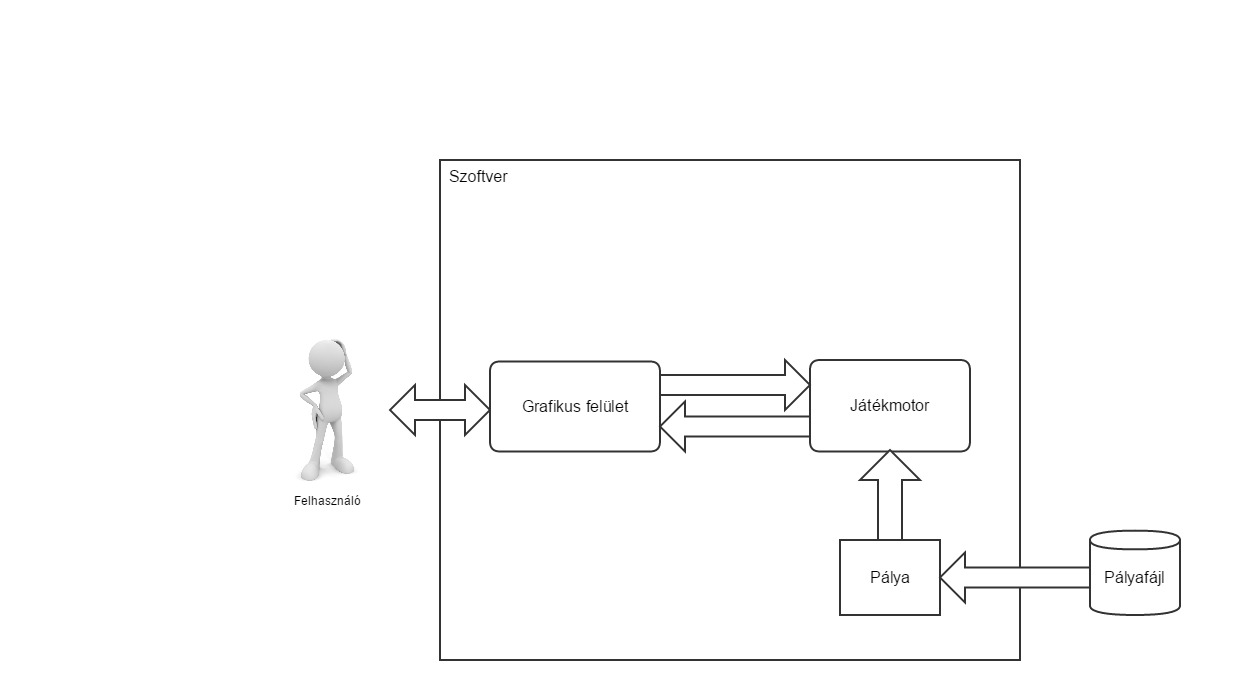
\includegraphics[width=180mm, center]{./chapters/chapter02/dia1.jpg}
	\caption{Architekturális kép \label{overflow}}
\end{figure}

A szoftverünk legfontosabb komponense a játékmotor. Itt zajlanak le a számítások, ez futtatja a logikát, ami érzékeli, hogy egy robot elhagyta a pályát, esetleg beleugrott egy ragacsba, vagy egy olajfoltba. A játékmotor feladata az is, hogy észrevegye, amikor vége van a játéknak, azaz lejárt az idő, vagy csak egy robot maradt a pályán. \\

A grafikus felület a felhasználó számára megjeleníti a játékot, valamint ezen keresztül tudja befolyásolni a játékmotorban történő eseményeket. \\

Az előre elkészített pályát egy külső fájlból érjük el, ezt tartja nyilván a Pálya modul. A játékmotor természetesen hozzáfér ehhez, hiszen neki kell eldöntenie a robotok kezdőpozícióját, valamint az előre legenerált ragacsok és olajfoltok elhelyezkedését. \\


%Ennek kell 4000 karakternek lennie, ennek a követelménynek megfelel. Ennek az az ára, hogy tűnhet neekd is úgy, mint ha 1-2 dolog ismtlődne benne. No ezt azzal védeném, hogy van például egy rovid kis bevezető (1. bekezdés), ott van néhány dolog említve nagyjábókl a játékról, s utána ezeket kifejtem kicsit bővebben, ezért tűnhet úgy az ismétlés. A mennyiséget nem igen kéne csökkenteni, ahol nagyon rossznak érzed, azt kérlek bommierenben próbáljuk meg megvitatni, s igyekszem megvédeni. Fogalmazási kuszaságok vannak benne bőven, azt javítsátok bátran, ha valami nagyon feltűnően rossz, azt szintén említsétek, hogy tanuljak belőle. - sgabor
\subsection{Funkciók}

A szoftver egy úgynevezett Phoebe versenyszimulátor, amelyben robotok versenyezhetnek egymással. Először álló helyzetből indulnak, mindegyik egy előre generált pozícióból. A játék körökre osztott. Minden kör egy iterációnak felel meg, így minden játékos egy körben maximum két dolgot tehet meg: ragacsot helyezhet el, vagy olajfoltot hagyhat maga után (a kettő közül természetesen csak az egyiket), valamint változtathatja a sebességét. A robotok egy előre elkészített versenypályán mozognak. A pályáról leugró robotok elakadnak és kiesnek a játékból.\\

A robotok sebessége egységnyi méretű, tetszőleges irányú sebességvektorral tetszőlegesen módosítható. Egy ugrással a sebességgel egyenesen arányos távolságra tudnak eljutni.\\

Az elején betöltődik a pálya, ami szabályos sokszögekből fog állni, majd véletlenszerűen generálódik rá néhány olaj -és ragacsfolt, valamint a játékosokhoz tartozó robotok. A játék csak többjátékos módban játszható és minden körben szépen sorban mindenki beállíthatja, hogy merre kívánja módosítani a robotjának a sebességét, és hogy kíván-e hátrahagyni valamilyen foltot. Ezután a megadott beállítások véglegesednek, s ennek megfelelően ugrik egyszerre az összes robot. Ha két - vagy több - robot ugyanarra a mezőre ugrik, akkor mindegyiket megpróbálja áthelyezni a játék egy véletlenszerűen választott üres szomszédos cellába, ha pedig ez nem lehetséges (mert a pálya széle, vagy az őket körülvevő robotok ezt lehetetlenné teszik), tehát ha nincs elegendő szabad cella az adott cella körül, akkor az összes érintett robot megsemmisül és ezáltal kiesik a játékból.\\

Ha a robot olyan cellába ugrik, ahol már nem tart a pálya, akkor leesik és szintén kiesik a játékból. Ha már csak egy robot marad a pályán, akkor játék véget ér és az egyetlen fennmaradó robot irányítója nyert.\\

A játékot a következő sebességre hatással bíró funkciók nehezítik meg, s teszik izgalmassá a versenyzést: a pályán vannak (illetve elhelyezhetők) olajfoltok, amikre érkezve sebességmódosításra nincs mód, a robot az addigi sebességével fog továbbhaladni, illetve ragacsfoltok, amik a sebesség nagyságát megfelezik. A robotok fel vannak szerelve olaj és ragacskészlettel, amikből a játékos parancsára elugráskor tudnak maguk mögött hagyni egyet. Amelyik robot a legügyesebben gazdálkodik ezekkel a képességekkel, az nyilván könnyen előnyre tehet szert az ellenfeleivel szemben, garantálva a szórakozást. Összefoglalva a pályán keletkező lehetséges akadályok és az egyéb verseny kimenetelére hatással bíró tényezők a következőek:\\

\begin{itemize}
	\item Olajfolt: hatására a robot sebessége nem módosítható, azaz a következő ugrás sebességvektora meg fog egyezni az előző ugráséval. Ez a pálya elhagyásához vezethet, ami a robot számára a játék végét jelenti.
	
	\item A másik lehetséges folt a ragacs. Ez minden esetben megfelezi a robot sebességét, tehát lassító hatással bír. Az idő lejártához közeledve nyilvánvaló, hogy a ragacsba való belépés akár az első hely elvesztésével is járhat, ezért célszerű elkerülni.
	
	\item Lyukak: a pályán véletlenszerűen lyukak lesznek találhatóak, a pálya generálásának véletlenszerűségéből adódóan (a pálya nem feltétlen egy szabályosnak mondható alakzatot vesz majd fel, így szélein is egyenetlenségek keletkezhetnek majd). Ezekre a lyukas cellákra lépve a játék az adott robot számára szintén véget ér, mivel a robot letért a pályáról.
\end{itemize}

Mindenkinek lesz korlátozott számú foltja amit a pályára dobálhat. Egy cellán csak egyféle folt lehet, vagy üresen is állhat természetesen. Foltot már az első kör végén is hagyhatnak maguk után a robotok. A folt hatása a belelépő robot számára csak addig tart, amíg a robot el nem lép a "foltos" celláról. Ha egy robot belelép egy foltba, akkor a folt nem tűnik el, hogy később más is beleléphessen, így a foltos cellák száma sosem csökkenhet, ezzel is fenntartva a játék izgalmait.\\

Az olajfoltot vagy a ragacsot az ugrás előtt tudja maga mögött hagyni, természetesen ezt a felhasználó dönti el, hogy mikor alkalmazza. Legcélszerűbb akkor kiadni ezeket az utasításokat, amikor az ellenfél nagy eséllyel nem, vagy csak nehezen tudja elkerülni az ezen való áthaladást.\\

A játékot a következőképpen lehet megnyerni: az ellenfelek a fent leírt okok valamelyike miatt megsemmisülnek, s már csak egyetlen robot marad fenn a pályán; vagy az a robot nyer, amelyik a megadott idő -illetve körlimit letelte után a legnagyobb utat tette meg.\\

\subsection{Felhasználók}

A szoftver több felhasználóra van tervezve, akik számára a játék könnyedén elsajátítható, amennyiben ismerik a szótárban megnevezett definíciókat. Egyjátékos módra nincs lehetőség.

\subsection{Korlátozások}

Korlátozásként megfogalmazható az, hogy a forrásprogramnak a laboratóriumban rendszeresített JDK alatt lefordíthatónak és futtathatónak kell lennie, nem adható hozzá külső package.

\subsection{Feltételezések, kapcsolatok}

Szoftver labor 4 feladatkiírás: \textit{https://www.iit.bme.hu/$\sim$szoftlab4/feladat.shtml}

\section{Követelmények}


\subsection{Funkcionális követelmények}


% Azonosító, Leírás, Ellenőrzés, Prioritás, Forrás, Use-case, Komment
\begin{longtable}{| l | l | l | l | l | l | l |}
\hline
\textbf{Azonosító}   & \textbf{Leírás} & \textbf{Ellenőrzés} & \textbf{Prioritás} & \textbf{Forrás} & \textbf{Use-case} & \textbf{Komment} \tabularnewline
\hline\hline
1.01 & Absztrakt pálya & bemutatás & fontos & megrendelő & Main use-case & komment \tabularnewline
\hline
1.02 & Robot irányító felület & bemutatás & fontos & megrendelő & Main use-case & komment \tabularnewline
\hline
1.03 & Egy robot mozog a pályán & bemutatás & fontos & megrendelő &  & komment \tabularnewline
\hline
1.04 & Távolság számítása & bemutatás & alapvető & megrendelő & Eredmény use-case & komment \tabularnewline
\hline
1.05 & A robot leesik a pályáról & bemutatás & alapvető & megrendelő &  & komment \tabularnewline
\hline
1.06 & Játék vége & bemutatás & fontos & megrendelő & Eredmény use-case & Megadott idő/kör után vagy ha a robot leesik a pályáról \tabularnewline
\hline
1.07 & Eredmény kiírása, új játék & bemutatás & fontos & megrendelő & Eredmény use-case & komment \tabularnewline
\hline
1.08 & A robot foltba megy& bemutatás & alapvető & megrendelő &  & komment \tabularnewline
\hline
1.09 & Robot foltkészlete & bemutatás & opcionális & csapat & Main use-case & komment \tabularnewline
\hline
1.10 & A robot felszedi a foltokat & bemutatás & opcionális & csapat &  & komment \tabularnewline
\hline
1.11 & A robot elhelyezi a foltokat & bemutatás & alapvető & megrendelő &  & komment \tabularnewline
\hline
1.12 & Több robot a pályán & bemutatás & fontos & megrendelő &  & komment \tabularnewline
\hline
1.13 & A robotok egymás után jönnek & bemutatás & alapvető & megrendelő &  & komment \tabularnewline
\hline
1.14 & Menürendszer & bemutatás & opcionális & megrendelő & Menu use-case & komment \tabularnewline
\hline
\end{longtable}

\subsection{Erőforrásokkal kapcsolatos követelmények}

% Azonosító, Leírás, Ellenőrzés, Prioritás, Forrás, Komment
\begin{longtable}{| l | l | l | l | l | l |}
\hline
\textbf{Azonosító}   & \textbf{Leírás} & \textbf{Ellenőrzés} & \textbf{Prioritás} & \textbf{Forrás} & \textbf{Komment} \tabularnewline
\hline\hline
2.01 & Git & nincs & alapvető & csapat & Verziókezelés \tabularnewline
\hline
2.02 & GitHub & nincs & alapvető & csapat & Git tárhely \tabularnewline
\hline
2.03 & SourceTree & nincs & alapvető & csapat & Git GUI \tabularnewline
\hline
2.04 & Tex Studio & nincs & alapvető & csapat & Latex szerkesztő \tabularnewline
\hline
2.05 & JRE6 & nincs & fontos & megrendelő &  \tabularnewline
\hline
2.06 & Eclipse & nincs & alapvető & csapat & Java IDE  \tabularnewline
\hline
2.07 & Facebook & nincs & alapvető & csapat & Kapcsolattartás \tabularnewline
\hline
\end{longtable}


\subsection{Átadással kapcsolatos követelmények}


\begin{longtable}{| l | l | l | l | l | l |}
\hline
\textbf{Azonosító}   & \textbf{Leírás} & \textbf{Ellenőrzés} & \textbf{Prioritás} & \textbf{Forrás} & \textbf{Komment} \tabularnewline
\hline\hline
3.01 & Szkeleton átadás & bemutatás & fontos & megrendelő & márc. 23. \tabularnewline
\hline
3.02 & Proto átadás & bemutatás & fontos & megrendelő & márc. 23. \tabularnewline
\hline
3.03 & Grafikus átadás & bemutatás & fontos & megrendelő & márc. 23. \tabularnewline
\hline
3.04 & A programnak működnie kell a HSZK gépein & bemutatás & fontos & megrendelő & márc. 23. \tabularnewline
\hline
\end{longtable}

\subsection{Egyéb nem funkcionális követelmények}


% Azonosító, Leírás, Ellenőrzés, Prioritás, Forrás, Komment
\begin{longtable}{| l | l | l | l | l | l |}
\hline
\textbf{Azonosító}   & \textbf{Leírás} & \textbf{Ellenőrzés} & \textbf{Prioritás} & \textbf{Forrás} & \textbf{Komment} \tabularnewline
\hline\hline
4.01 & Jól nézzen ki a játék & nincs & opcionális & csapat & \tabularnewline
\hline
\end{longtable}




\section{Lényeges use-case-ek}
\comment{A 2.3.1-ben felsorolt követelmények közül az alapvető és fontos követelményekhez tartozó használati esetek megadása az alábbi táblázatos formában.}
\subsection{Use-case leírások}

\comment{Minden use-case-hez külön}

\usecase{...}{...}{...}{...}

\usecase{...}{...}{...}{...}

\section{Szótár}
\comment{A szótár a követelmények alapján készítendő fejezet. Egy szótári bejegyzés definiálásához csak más szótári bejegyzések és köznapi – a feladattól független – fogalmak használhatók fel. A szótár mérete kb. 1-2 oldal legyen.}

\section{Projekt terv}
\subsection{Projekt terv}
\subsubsection{Csapat}
A csapat öt főből áll, próbálunk mindenkinek azonos nehézségű feladatokat találni, 
ami lehetőleg megfelel az egyéni preferenciáinak, nincsenek dedikált szerepek, mindenki foglalkozik mindennel.

\begin{center}
	\begin{tabular}{ | c | c | }
	\hline
		\multicolumn{2}{ | c | }{
			\textbf{Stapelspeicher csapat}} \\ \hline
		\textbf{Név} & 
		\textbf{Feladatkör} 
		\\ \hline \hline
		Kemény Károly & the boss \\ \hline
		Gema Barnabás &  cickány \\ \hline
		Juszt Ádám & the punctual \\ \hline
		Somogyi Gábor & the loud guy \\ \hline
		Pilinszki-Nagy Csongor & the manager \\ \hline
		
		
	\end{tabular}
\end{center}

\subsubsection{Kommunikáció}

\paragraph{verziókezelés} Verziókezelésre a csapat a Git nevű verziókezelő rendszerre épülő Github platformot használja, azért mert ingyenes, elterjedt, és kiváló szolgáltatások épülnek köré. Így tartja nyilván a csapat a dokumentáció illetve a forráskód inkrementális változásait.

\paragraph{facebook} A csapat egy privát facebook csoportot használ fórum jelleggel, ide kerülnek ki, és innen kereshetőek vissza a közérdekű információk, például a megbeszélések időpontjai.

\paragraph{megbeszélések} A különböző feladatrészek a megbeszéléseken kerülnek kiosztásra, amiket úgy tervezünk, hogy lehetőleg mindenki részt tudjon venni rajta személyesen. Ezen felül még folytatunk skype megbeszéléseket is.

\subsubsection{Használt Programok}

\paragraph{Verziókezelés} Verziókezelésre Git programot használunk, a main repositoryt a Github szolgáltatja, amely egyszerűvé teszi a kollaborálást.

\paragraph{Fejlesztőkörnyezet} Fejlesztéshez a csapat Eclipset illetve IntelliJ IDEA-t használ.

\paragraph{Dokumentáció} Dokumentációra LaTeX-et használunk. A szerkesztő környezetként a TeXstudio nevű szoftver szolgál, illetve az egész dokumentáció a projekttel együtt egy repositoryban verziókezelés alatt áll.

\subsubsection{Mérföldkövek, Határidők}

\begin{center}
	\begin{tabular}{ | l | l | l | }
		\hline
		\textbf{Dátum} &
		\textbf{Feladat} &
		\textbf{Ellenőrzés}
		
		\\ \hline \hline
		febr. 23. & Követelmény, projekt, funkcionalitás & beadás
		\\ \hline 
		márc. 2. &	Analízis modell kidolgozása 1. & beadás
		\\ \hline 
		márc. 9. &	Analízis modell kidolgozása 2. & beadás
		\\ \hline 
		márc. 16. &	Szkeleton tervezése & beadás
		\\ \hline 		
		márc. 23. &	Szkeleton & beadás
		\\ \hline
		márc. 25. & Szkeleton & bemutató
		\\ \hline 
		márc. 30. &	Prototípus koncepciója & beadás
		\\ \hline 
		ápr. 7.	 & Részletes tervek & beadás
		\\ \hline 
		ápr. 20. &	Prototípus & beadás
		\\ \hline 
		ápr. 22. & Prototípus & bemutató
		\\ \hline
		ápr. 27. &	Grafikus felület specifikációja & beadás
		\\ \hline 	 
		máj. 11. &	Grafikus változat & beadás
		\\ \hline
		máj. 13. & Grafikus bemutató & bemutató
		\\ \hline
		máj. 15. &	Összefoglalás & beadás
		\\ \hline 
	\end{tabular}
\end{center}

\paragraph{Szkeleton változat} A szkeleton változat célja annak bizonyítása, hogy az objektum és dinamikus modellek a definiált feladat egy modelljét alkotják. A szkeleton egy program, amelyben már valamennyi, a végső rendszerben is szereplő business objektum szerepel. Az objektumoknak csak az interfésze definiált. Valamennyi metódus az indulás pillanatában az ernyőre szöveges változatban kiírja a saját nevét, majd meghívja azon metódusokat, amelyeket a szolgáltatás végrehajtása érdekében meg kell hívnia. Amennyiben a metódusból valamely feltétel fennállása esetén hívunk meg más metódusokat, akkor a feltételre vonatkozó kérdést interaktívan az ernyőn fel kell tenni és a kapott válasz alapján kell a továbbiakban eljárni. A szkeletonnak alkalmasnak kell lenni arra, hogy a különböző forgatókönyvek és szekvencia diagramok ellenőrizhetők legyenek. Csak karakteres ernyőkezelés fogadható el, mert ez biztosítja a rendszer egyszerűségét.

\paragraph{Prototípus} A prototípus program célja annak demonstrálása, hogy a program elkészült, helyesen működik, valamennyi feladatát teljesíti. A prototípus változat egy elkészült program kivéve a kifejlett grafikus interfészt. A változat tervezési szempontból elkészült, az ütemezés, az aktív objektumok kezelése megoldott. A business objektumok - a megjelenítésre vonatkozó részeket kivéve - valamennyi metódusa a végleges algoritmusokat tartalmazza. A megjelenítés és működtetés egy alfanumerikus ernyőn követhető, ugyanakkor a megjelenítés fájlban is logolható, ezzel megteremtve a rendszer tesztelésének lehetőségét. Különös figyelmet kell fordítani az interfész logikájára, felépítésére, valamint arra, hogy az mennyiben tükrözi és teszi láthatóvá a program működését, a beavatkozások hatásait.

\paragraph{Grafikus} A grafikus (teljes) változat a prototípustól elvileg csak a kezelői felület minőségében különbözhet. Ennek
változatnak az értékelésekor a hangsúlyt sokkal inkább a megvalósítás belső szerkezetére, semmint a külalakra
kell helyezni.


